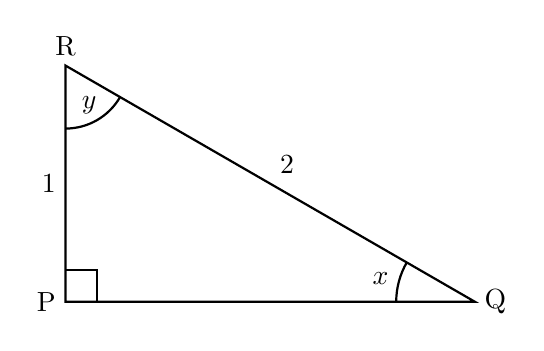
\begin{tikzpicture}[scale=1.0]

    % --- Define Coordinates ---
    % Point P at the origin (90 degree corner)
    \coordinate (P) at (0,0);
    
    % Point R on the y-axis. 
    % We choose a scale where length 1 = 3cm for visibility.
    \coordinate (R) at (0, 3);
    
    % Point Q on the x-axis.
    % Based on the labels, PR=1 and Hypotenuse RQ=2.
    % This is a 30-60-90 triangle.
    % If PR (height) = 3 units, then RQ (hypotenuse) = 6 units.
    % Then PQ (base) = sqrt(6^2 - 3^2) = sqrt(27) approx 5.2 units.
    \coordinate (Q) at (5.2, 0);

    % --- Draw Lines ---
    % Draw the triangle sides
    \draw[thick] (P) -- (Q) -- (R) -- cycle;

    % --- Labels for Vertices ---
    \node[left] at (P) {P};
    \node[right] at (Q) {Q};
    \node[above] at (R) {R};

    % --- Side Measurements ---
    % Label '1' for side PR
    \node[left] at (0, 1.5) {1};
    
    % Label '2' for side RQ (hypotenuse)
    \node[above right] at (2.6, 1.5) {2};

    % --- Right Angle Symbol ---
    % Draw a small square at P to indicate 90 degrees
    \draw[thick] (0, 0.4) -- (0.4, 0.4) -- (0.4, 0);

    % --- Angles and Labels ---
    
    % Angle at R (top, labeled 'y')
    % The vertical line is at 270 degrees relative to R.
    % The hypotenuse is at approx 330 degrees relative to R.
    \draw[thick] (0, 2.2) arc (270:330:0.8);
    \node at (0.3, 2.5) {$y$};

    % Angle at Q (bottom right, labeled 'x')
    % The horizontal line is at 180 degrees relative to Q.
    % The hypotenuse is at 150 degrees relative to Q.
    \draw[thick] (4.2, 0) arc (180:150:1.0);
    \node at (4.0, 0.3) {$x$};

\end{tikzpicture}